\documentclass[a4paper]{article}

%% Language and font encodings
\usepackage[english]{babel}
\usepackage[utf8x]{inputenc}
\usepackage[T1]{fontenc}

%% Sets page size and margins
\usepackage[a4paper,top=3cm,bottom=2cm,left=3cm,right=3cm,marginparwidth=1.75cm]{geometry}

% packages
\usepackage{amsmath, amsfonts}
\usepackage{graphicx, multicol}
\usepackage{textgreek,mathrsfs,bbm,relsize,multirow,float}
\usepackage{amssymb,amsthm,mathtools,scrextend,stackengine}
\usepackage[table,xcdraw]{xcolor} % clashes with tikz package
\usepackage[colorinlistoftodos]{todonotes}
\usepackage{url}
\usepackage{wrapfig}
\newenvironment{frcseries}{\fontfamily{frc}\selectfont}{}
%% commands
\newcommand{\xbar}{\mbox{\larger$\bar{x}$}}
\renewcommand{\baselinestretch}{1.5} %%1.5 spacing
\newcommand{\textfrc}[1]{{\frcseries#1}}
% commands

\newenvironment{sbmatrix}[1]
 {\def\mysubscript{#1}\mathop\bgroup\begin{bmatrix}}
 {\end{bmatrix}\egroup_{\textstyle\mathstrut\mysubscript}}
 
\pgfdeclarelayer{background}
\pgfsetlayers{background,main}

\title{Stats Learning Lecture Week 7}

\begin{document}
\section{Week 7 - Notes}

This week, chapter 6 in the ISLR book and chapter 3 in Intro to ML in Python would be handy read along guides to dimensionality reduction.

* have R code for pca/nmf in yale data set

So you've finally made it big time and got your hands on some Big Data\textsuperscript{TM}. Great! But where do you even start? You suddenly have more variables than you can count and no way to possibly check the importance of every variable. While you could use regularization methods like LASSO to try to curb how many variables affect your model, another technique is to reduce the dimensionality of the data- that is to linearly combine variables into a new super variable. By doing this, you  can keep the most important features of your data set while still greatly reducing the number of variables you keep. One common method of dimensionality reduction is called principal component analysis- or PCA. This is very useful for facial recognition software. 

Remember in week 2 when we read in images to R and played around with them? As you'll recall, the Crosby image was the largest image we used and had a clear difference in display and computation speed than the Lena photo which was both much smaller and already in grayscale. Now think to any crime show on TV- they always have a moment where they run facial recognition on someone from a CCTV camera and somehow \textit{their} software runs much faster even though they have a million times more faces. While Hollywood does exaggerate the computational ability of computers, there is some truth to what they do. Generally, facial recognition software is run with some form of dimensionality reduction, like PCA, to greatly decrease the computational time. 

Mathematically, this means that the goal of PCA is to construct a mapping between the original image to a new reduced image such that:

$$\underset{(p\times n)}{x} \mapsto \underset{(q\times n)}{z}$$

where $q<<<p$ and $q\leq n$. Take note that you cannot reduce the dimensionality to be fewer than the number of rows in the original data! By doing PCA, we greatly reduce the dimensionality of our data but still give the same variance, covariance, or correlation structures the original data had. This is accomplished because the variance of our data is the maximum variance explained by any linear combination of the variables. Assuming $\sum_{i=1}^{n}x_{i}=\underset{p\times 1}{0}$ (aka, the data is centered such that the mean is 0 by standardizing the data), PCA follows as below:

\begin{enumerate}
\item Compute $C=\frac{1}{n}\sum_{i=1}^{n}x_{i}x_{i}^{T}$
\item Solve spectral decomposition (SVD) such that \begin{align*}
Cw_{j} &= \lambda_{j}w_{j} \text{ for } j=1,\dots,p\\
C&= W\wedge W^{T}=\sum_{j=1}^{p}\lambda_{j}w_{j}w_{j}^{T}
\end{align*}
Where $W_{j}$ are the eigenvectors of $C$ and $w_{j}$ are the principal components
\item Set q by selecting the percent of variation you want to be able to explain
\item Project $z=XW$
\item reconstruct $\hat{x}=LL^{T}X$
\end{enumerate}

The process of choosing the number of principal components to use can be done 2 different ways. Either you choose the percent of variation you want to capture ahead of time and find how many PCs that takes or you can plot out the PCs and find the "bend" or "elbow" in the scree plot (shown below). A scree plot shows you how much variation each additional principal component explains. In most cases, when you use a scree plot you would choose the number of components 

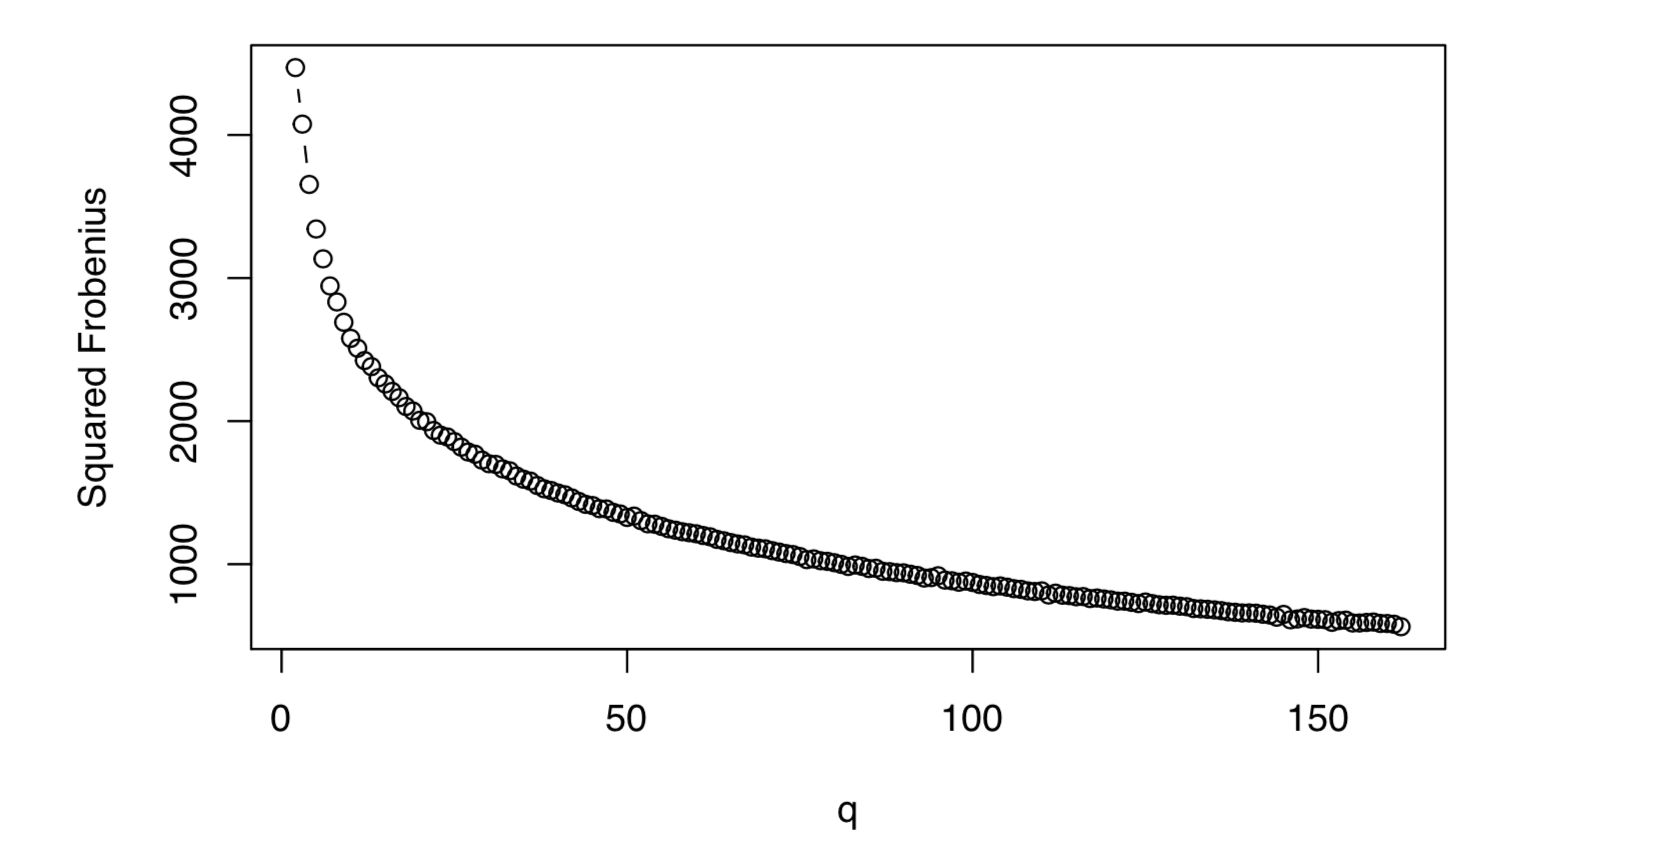
\includegraphics[scale=.6]{scree.png}

Let's say you do PCA, but end up needing nearly all of the $p$ principal components. Perhaps you'd have better luck reducing dimensionality if you used kernelized PCA instead. In kernelized PCA, we use the kernel $\Phi(x_{i})$ instead of $x_{i}$. In this way, we increase the dimensionality to find a pattern to be able to then greatly reduce dimensionality.
** GIF OF HOUSE FOR PICTURING KERNELS AGAIN

Another important aspect of kernerlized PCA, is that it allows you reduce dimesionality of non-continuous data. That is, if your data $X$ has categorical, ordinal variables, then you need only define a kernel for such data and can then perform PCA.

Non-Negative Matrix Factorization (NMF) works very similarly to PCA with one key difference. In PCA, we want our principal components to explain as much of the variation in the data as possible and this is accomplished by the eigenvectors being orthogonal.In NMF, we want our components to be positive (thus why it is \textbf{Non}-Negative Matrix Factorization). This difference may not seem important but it turns out that it makes NMF powerful at decomposing images and sounds that are overlayed/have multiple layers. In sound, this means NMF can decompose clips of multiple people speaking and have components that are easier to interpret than PCA. Check out the R code for this week to see how PCA and NMF differ in decomposing faces!

\section{SVD}
\subsection{Why SVD is important in Data Science}

When it comes to data science, a common case is that we need to deal with matrices and linear algebra problems. (Think of the data as a matrix with rows as observations and columns as attributes.) \\

A typical problem facing the Data Scientist is that the matrix is often of high dimension. It is natural to try to reduce the dimension of the matrix, also decompose the matrix (factorization) which will bring some nice properties when operating matrix calculation.\\ 

Singular Value Decomposition is a method of matrix factorization in linear algebra. It can be seen as a generalization of eigenvalue decomposition, in which the raw matrix must be square.\\ 

\subsection{Mathematics}

If matrix A has a dimension of $ n \times p $  and  $ n>p $, then $A$ can be decomposed as the following form:\\

\begin{equation}
A = UDV^{T}
\end{equation}
Dimensions:\\
$A:  n\times p$ \\
$U:  n\times m$ \\
$D:  n\times p$ \\
$V:  p\times p$ \\

\noindent Among which, the matrix have some nice properties.\\

\noindent Both $U$ and $V$ are orthogonal matrix (yes, that means they are square matrix as well), so that:
\newline
\\
\begin{eqnarray}
UU^{T} &=& I, \\
VV^{T} &=& I. 
\end{eqnarray}

$D$ is diagonal matrix, either square or not, with all the entries are the original matrix singular values, which are all non-negative. \\
\begin{equation}
DD^{T} = D^{2}.
\end{equation}

\subsection{SVD and PCA}

Now we should bring up the interesting part of matrix operation: \\
\begin{eqnarray}
\nonumber AA^{T} &=&  UDV^{T}(UDV^{T})^{T}, \\
\nonumber & = & UDV^{T}VD^{T}U^{T},  \\
 & = & UD^{2}U^{T}.
\end{eqnarray}

Since $ AA^{T} $ is used to calculate the covariance matrix in PCA, by eigenvalue decomposition, all the columns of $U$ are the eigenvectors of $AA^{T}$, and all the entries on $ S^{2} $ diagonal are the eigenvalues of $AA^{T}$. \\

\subsection{Applications of SVD}
\noindent SVD is widely used in all kinds of machine learning, engineering, data preprocessing. One example currently used by researchers at Notre Dame is in the merging of multiple 3D point-clouds obtained by scanning Heritage sites, such as the Taj Mahal. To generate a transformation from one point-cloud to another requires the coordinates of at least 3 points that can be identified in each point-cloud. Generally it is advantageous to have more than 3 point to minimize errors arising from the measurement of each point. SVD provides a way of solving this over-defined problem and reduces to a least-mean-squares fit for the point set. In general, the least square algorithm of linear regression could be simplified when SVD is applied to it. \\

\subsection{Intuitive interpretations}
\begin{figure}[H]
\center
\includegraphics[width=8cm]{intuitive_svd.png}
\caption{Intuitive interpretation of SVD.}
\label{svd}
\end{figure}
Visualization of the SVD decomposition of a two-dimensional, real shearing matrix $M$. In the above diagram the blue disc represents the unit circle and the arrows the two canonical unit vectors. The action of $M$ on the unit circle transforms it to an ellipse. The SVD decomposition of $M$ separates the transformation into  $V^*$, and initial rotation, $\Sigma$ a scaling along the coordinate axes and $U$ a final rotation. The lengths of the semi-axes of the ellipse, $\sigma_1$ and $\sigma_2$, are the singular values of $M$ represented by component $\Sigma_{1,1}$ and $\Sigma_{2,2}$.$^1$


\section{Citations}
[1] \url{https://ipfs.io/ipfs/QmXoypizjW3WknFiJnKLwHCnL72vedxjQkDDP1mXWo6uco/wiki/Singular_value_decomposition.html}


\end{document}
